% figures-es/littles-law.tex
% Standalone TikZ: ilustración de cola/pipeline de la Ley de Little L = lambda * W (ch.17).
\documentclass[tikz,border=4pt]{standalone}
\usepackage{tikz}
\usetikzlibrary{arrows.meta,positioning,calc}

\definecolor{vcblue}{HTML}{1A5276}
\definecolor{vcteal}{HTML}{0E6655}
\definecolor{vcgray}{HTML}{555555}

\begin{document}
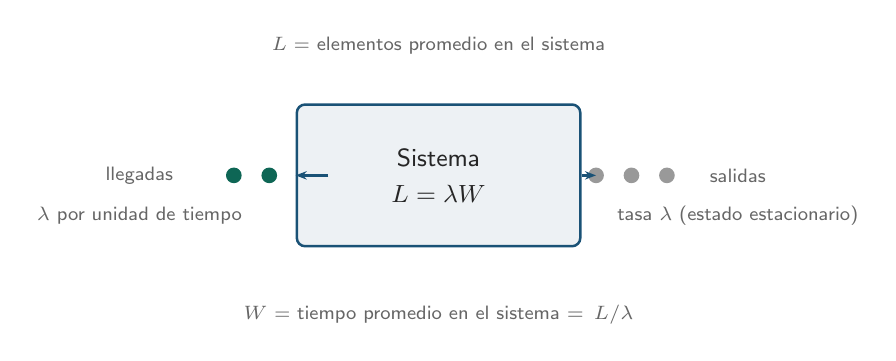
\begin{tikzpicture}[
  node distance=14mm,
  box/.style={
    draw=vcblue, line width=0.9pt, rounded corners=3pt,
    fill=vcblue!8, font=\sffamily\small, text=black!85,
    align=center, minimum width=36mm, minimum height=18mm
  },
  label/.style={font=\sffamily\scriptsize, text=black!60},
  arrow/.style={-{Stealth[length=4pt]}, vcblue, line width=0.9pt},
]

  % Flujo de llegadas (izquierda)
  \node[label] (arrlbl) at (-3.8, 0) {llegadas};
  \node[label, below=0.5mm of arrlbl] (arreq)  {\(\lambda\) por unidad de tiempo};

  % Puntos que representan llegadas
  \foreach \i in {0,1,2} {
    \node[circle, fill=vcteal, inner sep=2pt] (dot\i) at (-2.6 + \i*0.45, 0) {};
  }

  % Caja del sistema
  \node[box] (sys) at (0,0) {Sistema\\[2pt]\(\displaystyle L = \lambda W\)};

  % Flujo de salidas (derecha)
  \node[label] (deplbl) at (3.8, 0) {salidas};
  \node[label, below=0.5mm of deplbl] (depeq) {tasa \(\lambda\) (estado estacionario)};

  % Puntos que representan salidas
  \foreach \i in {0,1,2} {
    \node[circle, fill=vcgray!60, inner sep=2pt] (ddot\i) at (2.0 + \i*0.45, 0) {};
  }

  % Flechas de entrada y salida del sistema
  \draw[arrow] (-1.4, 0) -- (sys.west);
  \draw[arrow] (sys.east) -- (2.0, 0);

  % Anotación W debajo de la caja
  \node[label, below=6mm of sys] (wlbl)
    {\(W\) = tiempo promedio en el sistema \(=\, L / \lambda\)};

  % Anotación L arriba de la caja
  \node[label, above=5mm of sys] {\(L\) = elementos promedio en el sistema};

\end{tikzpicture}
\end{document}
